\documentclass{article}
\usepackage{graphicx}
\usepackage{amsthm}
\usepackage{amsmath}
\usepackage{amssymb}
\usepackage{geometry}
\usepackage{tikz}
\usetikzlibrary{arrows}

\geometry{a4paper, total={170mm,257mm}, left=20mm, top=20mm}
\AtBeginEnvironment{align}{\setcounter{equation}{0}} 

\title{HW7 (CSCI-C241)}
\author{Lillie Donato}
\date{5 March 2024}

\begin{document}

\maketitle

\begin{enumerate}
    \item $A \times A = \{(1,1),(1,2),(1,3),(2,1),(2,2),(2,3),(3,1),(3,2),(3,3)\}$
    \item Question Two
    \begin{enumerate}
        \item True
        \item False
        \item True
        \item True
        \item False
        \item False
        \item False
        \item True
        \item True
        \item False
        \item $|B \times C| = 21$
        \item $|R| = 9$
        \item $\{1,2,3,4,5,6,7\}$
        \item $\{\text{"a"}, \text{"b"}, \text{"c"}\}$
        \item 0
        \item 21
    \end{enumerate}
    \item Question Three
    \begin{enumerate}
        \item
        \begin{enumerate}
            \item Not Reflexive, $\neg R(b, b)$
            \item Not Anti-Reflexive, $R(d, d)$
            \item Not Symmetric, $R(a, b)$ but $\neg R(b, a)$
            \item Anti-Symmetric, the only related pairs where the order does not "matter", are those that pairs of equal items.
            \item Transitive, if one node is related to another, and that node is related to a third, the first node will be related to the third.
        \end{enumerate}
        \item
        \begin{enumerate}
            \item Not Reflexive, $\neg S(4, 4)$
            \item Not Anti-Reflexive, $S(1, 1)$
            \item Not Symmetric, $S(2,4)$ but $\neg S(4,2)$
            \item Not Anti-Symmetric, $S(1,2)$ and $S(2,1)$ but $1 \neq 2$
            \item Not Transitive, $S(1,2)$ and $S(2,4)$ but $\neg S(1,4)$
        \end{enumerate}
        \item
        \begin{enumerate}
            \item Not Reflexive, $\neg T(a,a)$
            \item Not Anti-Reflexive, $T(d,d)$
            \item Not Symmetric, $T(a,b)$ but $\neg T(b,a)$
            \item Not Anti-Symmetric, $T(c,d)$ and $T(d,c)$ but $c \neq d$
            \item Not Transitive, $T(b,c)$ and $T(c,d)$ but $\neg T(b,d)$
        \end{enumerate}
        \item
        \begin{enumerate}
            \item Not Reflexive, $\neg Q(1,1)$
            \item Anti-Reflexive, the sum of any integer and itself, is always even.
            \item Symmetric, order does not affect the sum of two integers.
            \item Not Anti-Symmetric, $Q(1,2)$ and $Q(2,1)$ but $1 \neq 2$
            \item Not Transitive, $Q(1,2)$ and $Q(2,3)$ but $\neg Q(1,3)$
        \end{enumerate}
        \item
        \begin{enumerate}
            \item Not Reflexive, $\neg C(\text{"str"}, \text{"str"})$
            \item Anti-Reflexive, a proper substring of a string can never be related on itself.
            \item Not Symmetric, $C(\text{"car"}, \text{"racecar"})$ but $\neg C(\text{"racecar"}, \text{"car"})$
            \item Anti-Symmetric, this is technically true, as if one string is related to the other, the other cannot be related to the first.
            \item Transitive, if a string is a proper substring of another string and that other string is a proper substring of a third string, the first string will be a proper substring of the third string.
        \end{enumerate}
        \item
        \begin{enumerate}
            \item Not Reflexive, $\neg A(P \land \neg P, P \land \neg P)$
            \item Anti-Reflexive, because a formula will never be logically equivalent to its negation.
            \item Symmetric, because order does not affect the logical equivalence of two formulas.
            \item Not Anti-Symmetric, $A(P \leftrightarrow Q, P \oplus Q)$ and $A(P \oplus Q, P \leftrightarrow Q)$ but $P \leftrightarrow Q \neq P \oplus Q$
            \item Not Transitive, $A(P \leftrightarrow Q, P \oplus Q)$ and $A(P \oplus Q, P \leftrightarrow Q)$ but $\neg A(P \leftrightarrow Q, P \leftrightarrow Q)$
        \end{enumerate}
    \end{enumerate}
    \item Question Four
    \begin{enumerate}
        \item
        \begin{enumerate}
            \item Not Reflexive, $\neg X(\{\}, \{\})$
            \item Not Anti-Reflexive, $X(\{1\}, \{1\})$
        \end{enumerate}
        \item
        \begin{enumerate}
            \item Symmetric, the order of the sets does not affect the condition.
            \item Not Anti-Symmetric, $X(\{1,2,3\}, \{2,3,4\})$ and $X(\{2,3,4\}, \{1,2,3\})$, but $\{1,2,3\} \neq \{2,3,4\}$
        \end{enumerate}
        \item
        \begin{enumerate}
            \item Not Transitive, $X(\{1,2\}, \{2,3\})$ and $X(\{2,3\}, \{3,4\})$ but $\neg X(\{1,2\}, \{3,4\})$
        \end{enumerate}
    \end{enumerate}
    \item Question Five
    \begin{enumerate}
        \item $\mathbb{N}$ 
        \item $\mathbb{N}$
        \item $M$ is reflexive because a natural number $n$ is a multiple of itself.
        \item
        Claim: $M$ is anti-symmetric
        \begin{proof}
            \begin{align}
                &\text{Choose } x,y \in \mathbb{N} \text{ and Assume } M(x,y) \text{ and } M(y,x) \\
                &\text{Since } M(x,y) \text{ and } M(y,x) \text{, we know } x \text{ is a multiple of } y \text{ and } y \text{ is a multiple of } x \\
                &\text{Since } x \text{ is a multiple of } y \text{, there exists some } k \in \mathbb{N} \text{ such that } x = ky \\
                &\text{Since } y \text{ is a multiple of } x \text{, there exists some } j \in \mathbb{N} \text{ such that } y = jx \\
                &\text{Since } x = ky \text{ and } y = jx \text{, we know } y = jky \\
                &\text{Since } y = jky \text{, we know } 1 = jk \\
                &\text{Since } jk = 1 \text{, we know } j = 1 \text{ and } k = 1 \\
                &\text{Since } j = 1 \text{ and } k = 1 \text{, we know } x = 1y \\
                &\text{Since } x = 1y \text{, weknow } x = y \text{, therefore } M \text{ is anti-symmetric} 
            \end{align}
        \end{proof}
        \item
        Claim: $M$ is transitive
        \begin{proof}
            \begin{align}
                &\text{Choose } x,y,z \in \mathbb{N} \text{ and Assume } M(x, y) \text{ and } M(y, z) \\
                &\text{Since } M(x,y) \text{ and } M(y,z) \text{, we know } x \text{ is a multiple of } y \text{ and } y \text{ is a multiple of } z \\
                &\text{Since } x \text{ is a multiple of } y \text{, there exists some } k \in \mathbb{N} \text{ such that } x = ky \\
                &\text{Since } y \text{ is a multiple of } z \text{, there exists some } j \in \mathbb{N} \text{ such that } y = jz \\
                &\text{Since } x = ky \text{ and } y = jz \text{, we know } x = kjz \\
                &\text{Let } n = kj \text{, such that } n \in \mathbb{N} \\
                &\text{Since } x = kjz \text{, we know } x = nz \\
                &\text{Since } x = nz \text{, we know } x \text{ is a multiple of } z \text{, so } M(x, z) \text{, therefore } M \text{ is transitive}
            \end{align}
        \end{proof}
    \end{enumerate}
    \item Question Six
    \begin{enumerate}
        \item True
        \item False
        \item True
        \item True
        \item True
        \item True
        \item
        Claim: $E_5$ is reflexive
        \begin{proof}
            \begin{align}
                &\text{Choose } x \in \mathbb{Z} \\
                &\text{Since } x - x = 0 \text{ and } 0 \text{ is a multiple of any number, } 0 \text{ is a multiple of } 5 \\
                &\text{Since } 0 \text{ is a multiple of } 5 \text{, we know } E_5(x, x) \text{, therefore } E_5 \text{ is reflexive}
            \end{align}
        \end{proof}
        \item
        Claim: $E_5$ is symmetric
        \begin{proof}
            \begin{align}
                &\text{Choose } x,y \in \mathbb{Z} \text{ and Assume } E_5(x, y) \\
                &\text{Since } E_5(x, y) \text{, we know } x - y \text{ is a multiple of } 5 \\
                &\text{Let } z = y - x \text{, such that } z \in \mathbb{Z} \\
                &\text{Since } y - x = z \text{, we know } x-y = -z \\
                &\text{Since } -z \text{ is a multiple of } 5 \text{, we know } z \text{ must be a multiple of } 5
            \end{align}
        \end{proof}
        \item
        Claim: $E_5$ is transitive
        \begin{proof}
            \begin{align}
                &\text{Choose } x,y,z \in \mathbb{Z} \text{ and Assume } E_5(x, y) \text{ and } E_5(y, z) \\
                &\text{Since } E_5(x,y) \text{ and } E_5(y,z) \text{, we know } x - y \text{ is a multiple of } 5 \text{ and } y - z \text{ is a multiple of } 5 \\
                &\text{Let } a = x - y \text{ and } b = y - z \text{, such that } a,b \in \mathbb{Z} \\
                &\text{Since } a \text{ is a multiple of } 5 \text{ and } b \text{ is a multiple of } 5 \text{, we know } a + b \text{ must be a multiple of } 5 \\
                &\text{Let } n = a + b \text{, such that } n \in \mathbb{Z} \text{ and } n \text{ is divisible by } 5 \text{ because } a+b \text{ is a multiple of } 5 \\
                &\text{Since } n = a + b \text{, we know } n = (x-y) + (y-z) \\
                &\text{Since } n = (x-y) + (y-z) \text{, we know } n = x - y + y - z \\
                &\text{Since } n = x-y+y-z \text{, we know } n = x - z \\
                &\text{Since } n = x-z \text{, we know } x - z \text{ is divisible by } 5 \\
                &\text{Since } x - z \text{ is divisible by } 5 \text{, we know } E_5(x,z) \text{, therefore } E_5 \text{ is transitive}
            \end{align}
        \end{proof}
    \end{enumerate}
    \item Question Seven
    \begin{enumerate}
        \item $Q$ does not have property $F$, because $Q(a, 1)$ and $Q(a, 2)$ but $1 \neq 2$
        \item $L$ has property $F$, because a string $s$ will always have the same length.
        \item
        Claim: $I$ has property $F$
        \begin{proof}
            \begin{align}
                &\text{Choose } x,y,z \in \mathbb{R} \text{ and Assume } I(x,y) \text{ and } I(x,z) \\
                &\text{Since } I(x,y) \text{ and } I(x,z) \text{, we know } x \cdot y=x \cdot z \\
                &\text{Since } x \cdot y=x \cdot z \text{, we know } y=z \text{, therefore } I \text{ has property } F
            \end{align}
        \end{proof}
    \end{enumerate}
    \item Question Eight
    \begin{enumerate}
        \item $\{(a, a), (a, b), (b, a), (b, c), (c,d), (d,a)\}$ on $A$
        \item
        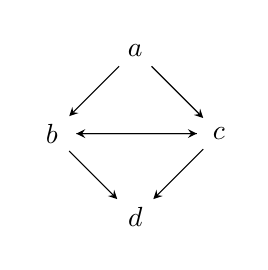
\begin{tikzpicture}[scale=1.5, node distance={15mm}, main/.style = {circle}]
            % Nodes
            \node[main] (1) {$a$};
            \node[main] (2) [below left of=1] {$b$};
            \node[main] (3) [below right of=1] {$c$};
            \node[main] (4) [below right of=2] {$d$};

            % Loops
            % \draw[->,>=stealth] (1) edge[out=120, in=60, looseness=5] (1);
            
            % Lines
            \draw[->,>=stealth] (1) -- (2);
            \draw[->,>=stealth] (1) -- (3);
            \draw[->,>=stealth] (2) -- (4);
            \draw[->,>=stealth] (3) -- (4);
            \draw[->,>=stealth] (2) -- (3);
            \draw[->,>=stealth] (3) -- (2);
            
        \end{tikzpicture}
        \item $\{(s,t) \mid s \text{ shares a character with } t\}$
        \item $\{(s,t) \mid |s| > |t|\}$
        \item $\{(x,y) \mid x+y=10\}$
        \item $\{(p,q) \mid p \equiv q\}$
        \item $\{(p,q) \mid p \text{ has more implication statements than } q\}$
        \item $\{(p,q) \mid \text{the name of } p \text{ is a substring of the name of } q \text{ but nobody else has the exact same name as } p \text{ or } q\}$
    \end{enumerate}
\end{enumerate}

\end{document}